%%%%%%%%%%%%%%%%%%%%%%%%%%%%%%%%%%%%%%
%%%%%%%%%%%%%%%%%%%%%%%%%%%%%%%%%%%%%%
% Do not edit the TeX file your work
% will be overwritten.  Edit the RnW
% file instead.
%%%%%%%%%%%%%%%%%%%%%%%%%%%%%%%%%%%%%%
%%%%%%%%%%%%%%%%%%%%%%%%%%%%%%%%%%%%%%




\newcommand{\BCLTDensitiesGraph}{
%<<mult_path, cache=cache, fig.show='hold', fig.cap=fig_cap>>=
\begin{knitrout}
\definecolor{shadecolor}{rgb}{0.969, 0.969, 0.969}\color{fgcolor}

{\centering 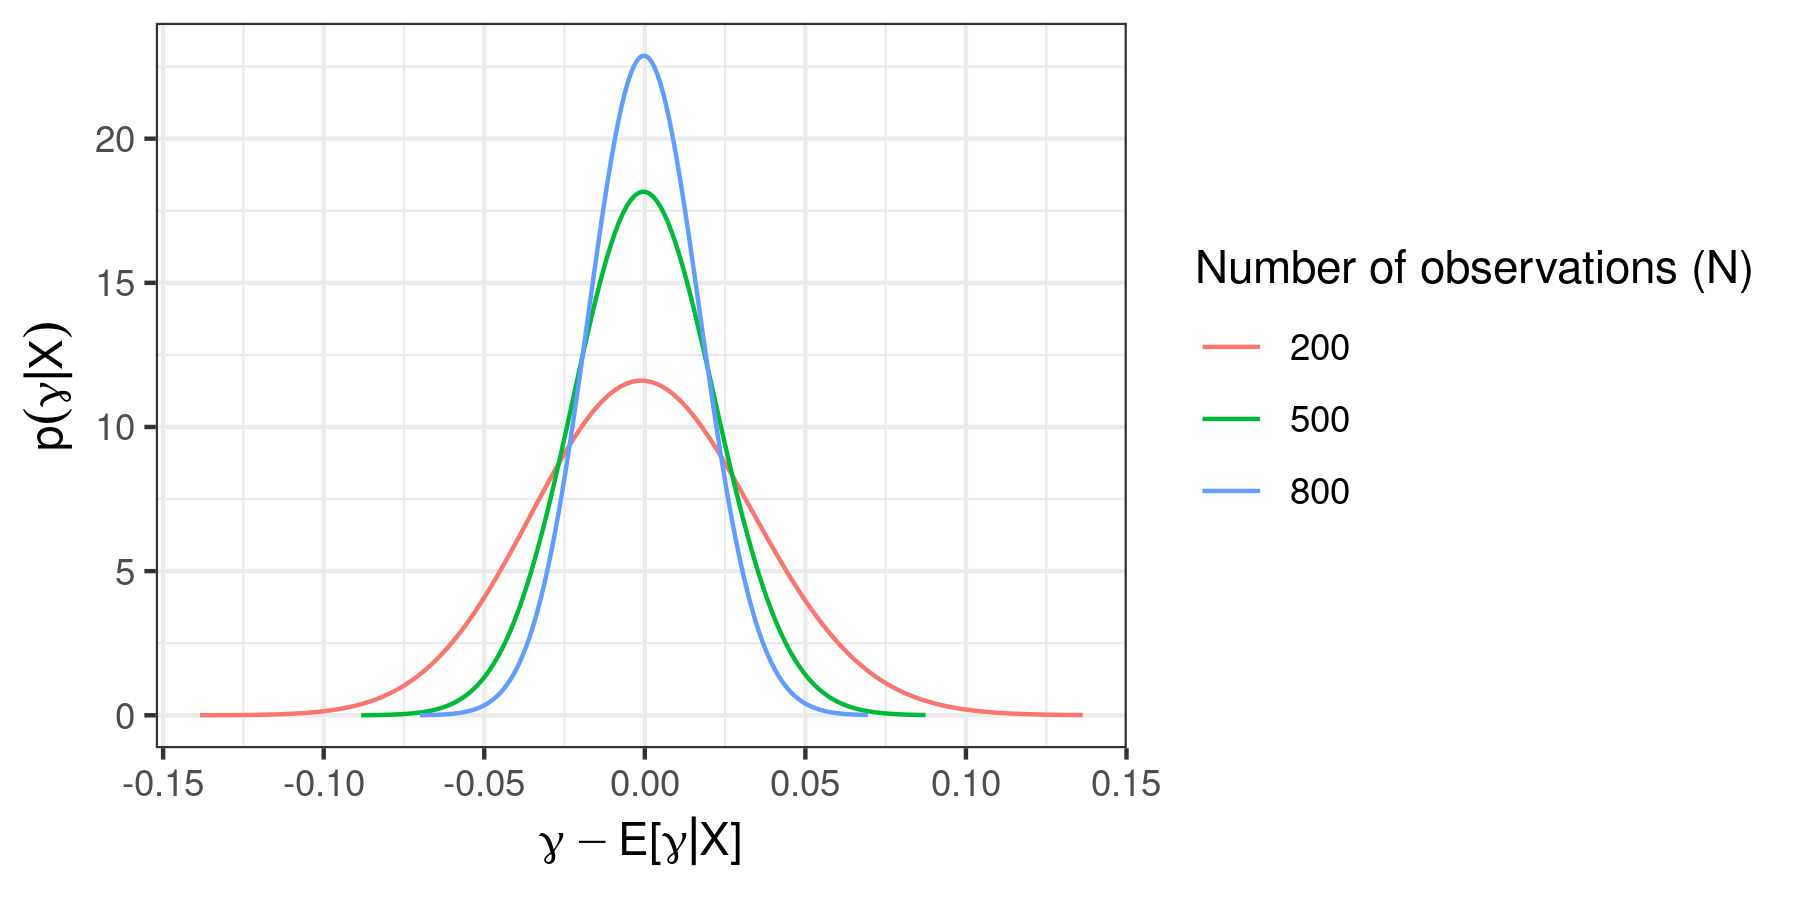
\includegraphics[width=0.980\linewidth,height=0.490\linewidth]{figure/bcltdensities-1} 

}



\end{knitrout}
}



\newcommand{\LowDimAccuracyGraph}{
%<<mult_path, cache=cache, fig.show='hold', fig.cap=fig_cap>>=
\begin{knitrout}
\definecolor{shadecolor}{rgb}{0.969, 0.969, 0.969}\color{fgcolor}

{\centering 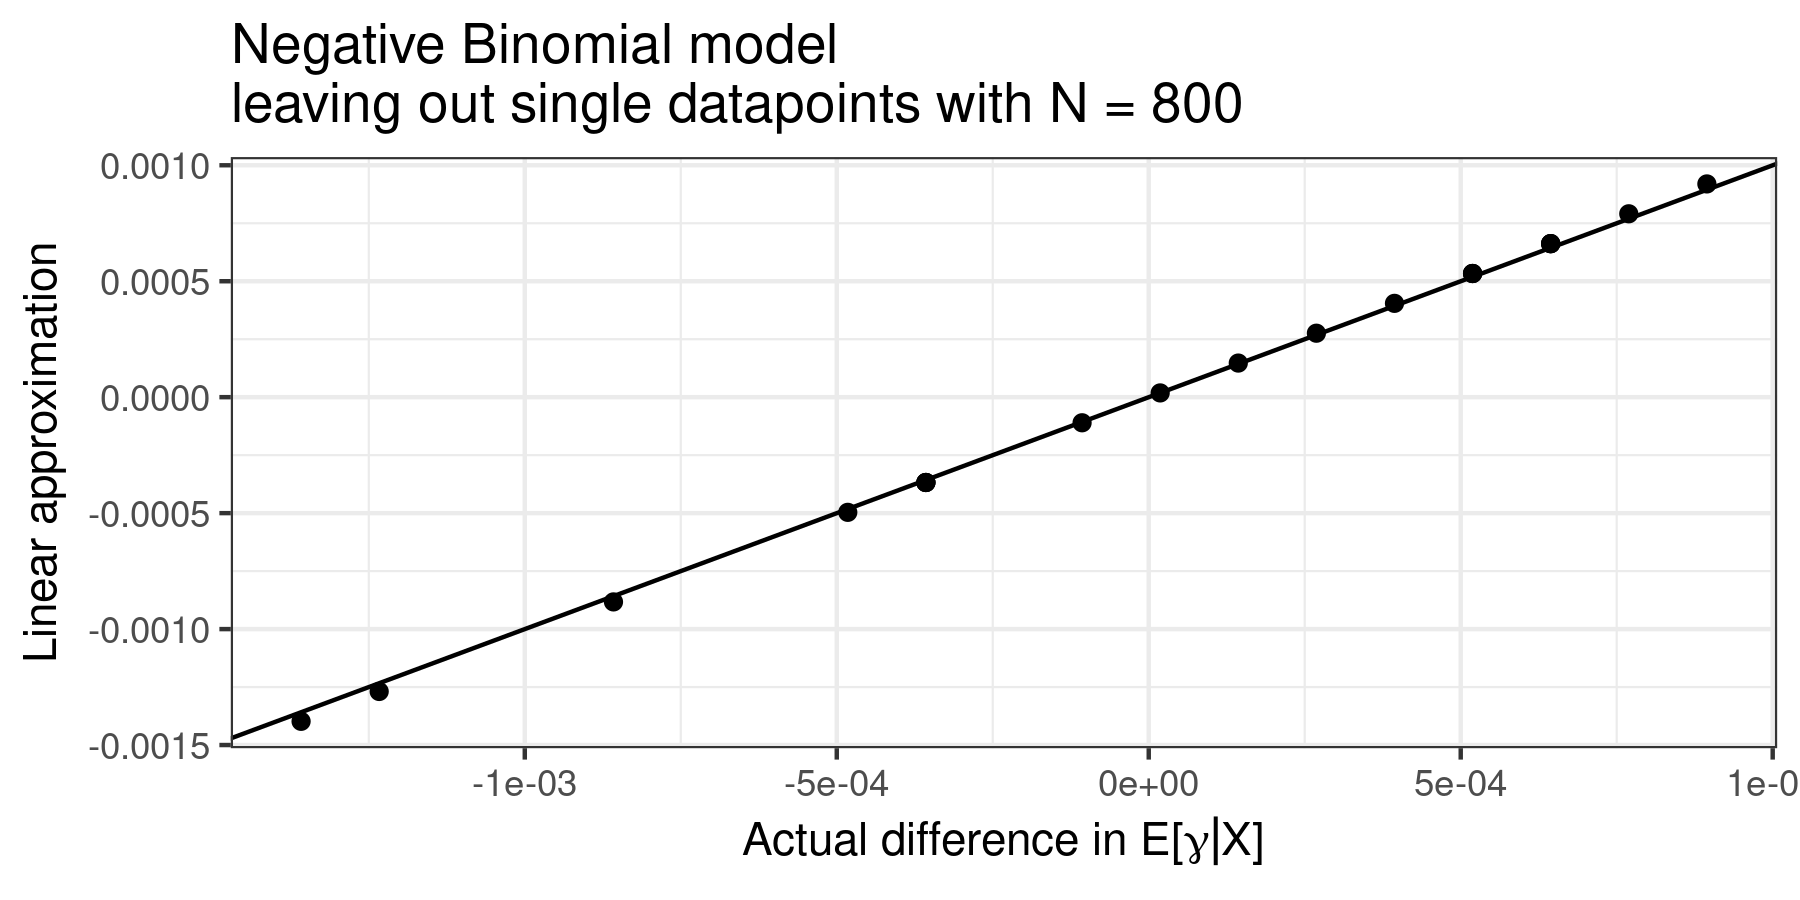
\includegraphics[width=0.980\linewidth,height=0.490\linewidth]{figure/lowdim_accuracy-1} 

}



\end{knitrout}
}



\newcommand{\HighDimAccuracyGraph}{
%<<mult_path, cache=cache, fig.show='hold', fig.cap=fig_cap>>=
\begin{knitrout}
\definecolor{shadecolor}{rgb}{0.969, 0.969, 0.969}\color{fgcolor}

{\centering 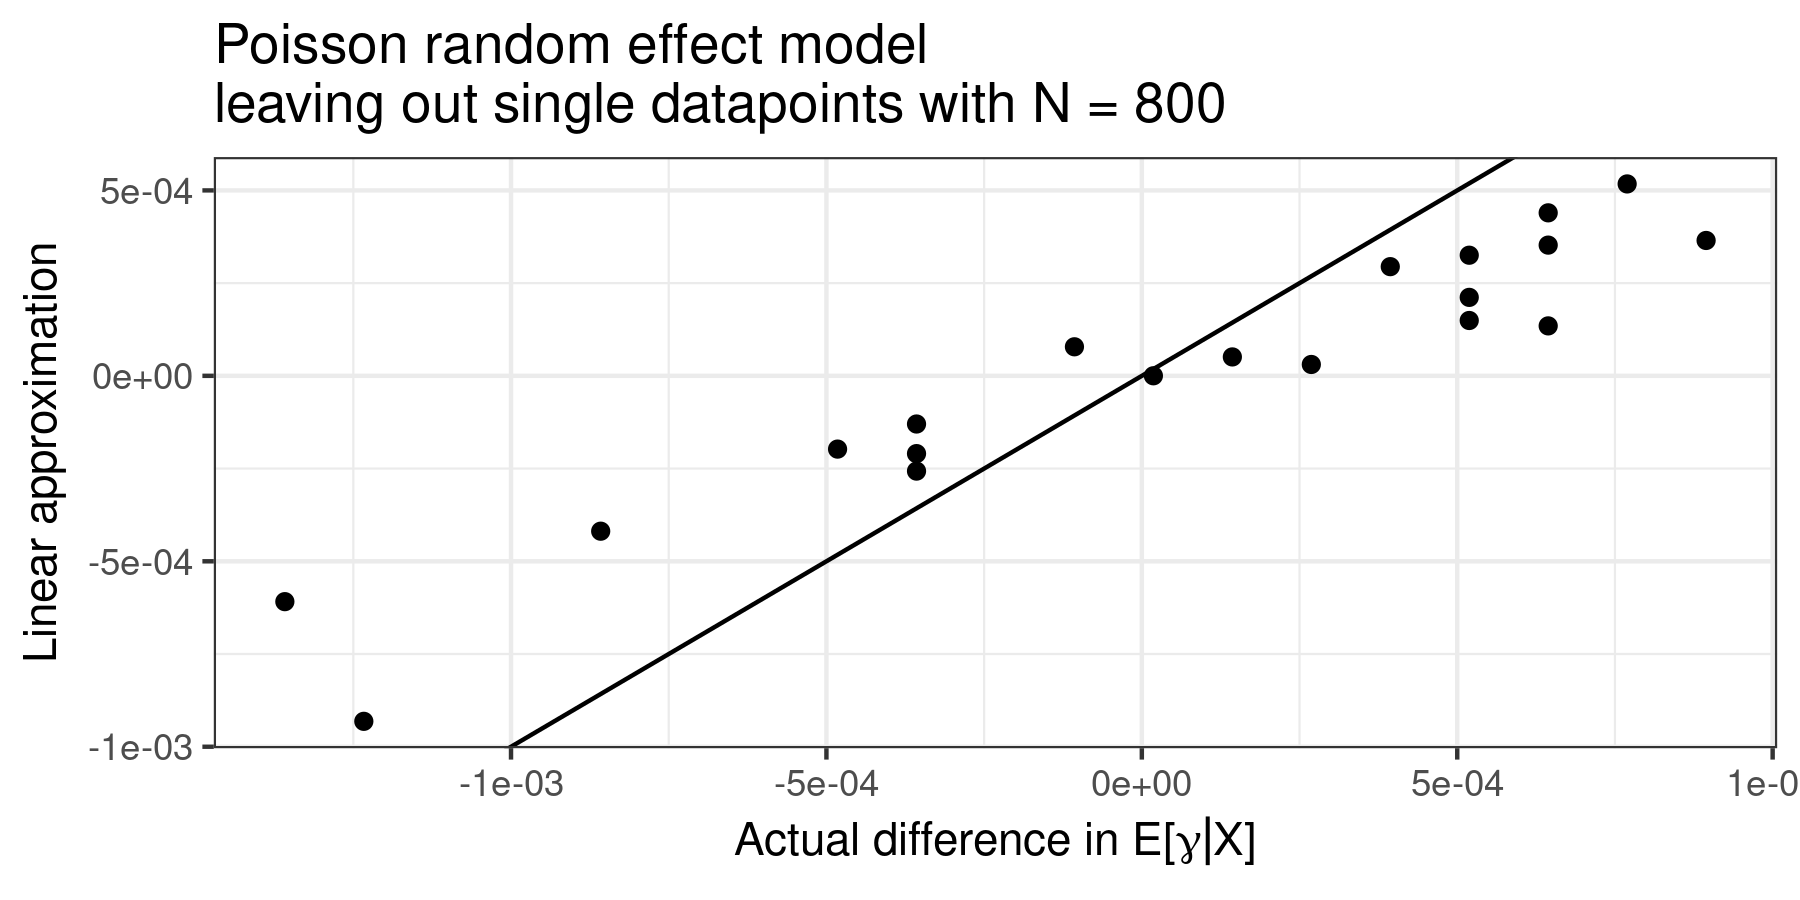
\includegraphics[width=0.980\linewidth,height=0.490\linewidth]{figure/highdim_accuracy-1} 

}



\end{knitrout}
}


\newcommand{\ManyPlotsOne}{
%<<mult_path, cache=cache, fig.show='hold', fig.cap=fig_cap>>=
\begin{knitrout}
\definecolor{shadecolor}{rgb}{0.969, 0.969, 0.969}\color{fgcolor}

{\centering 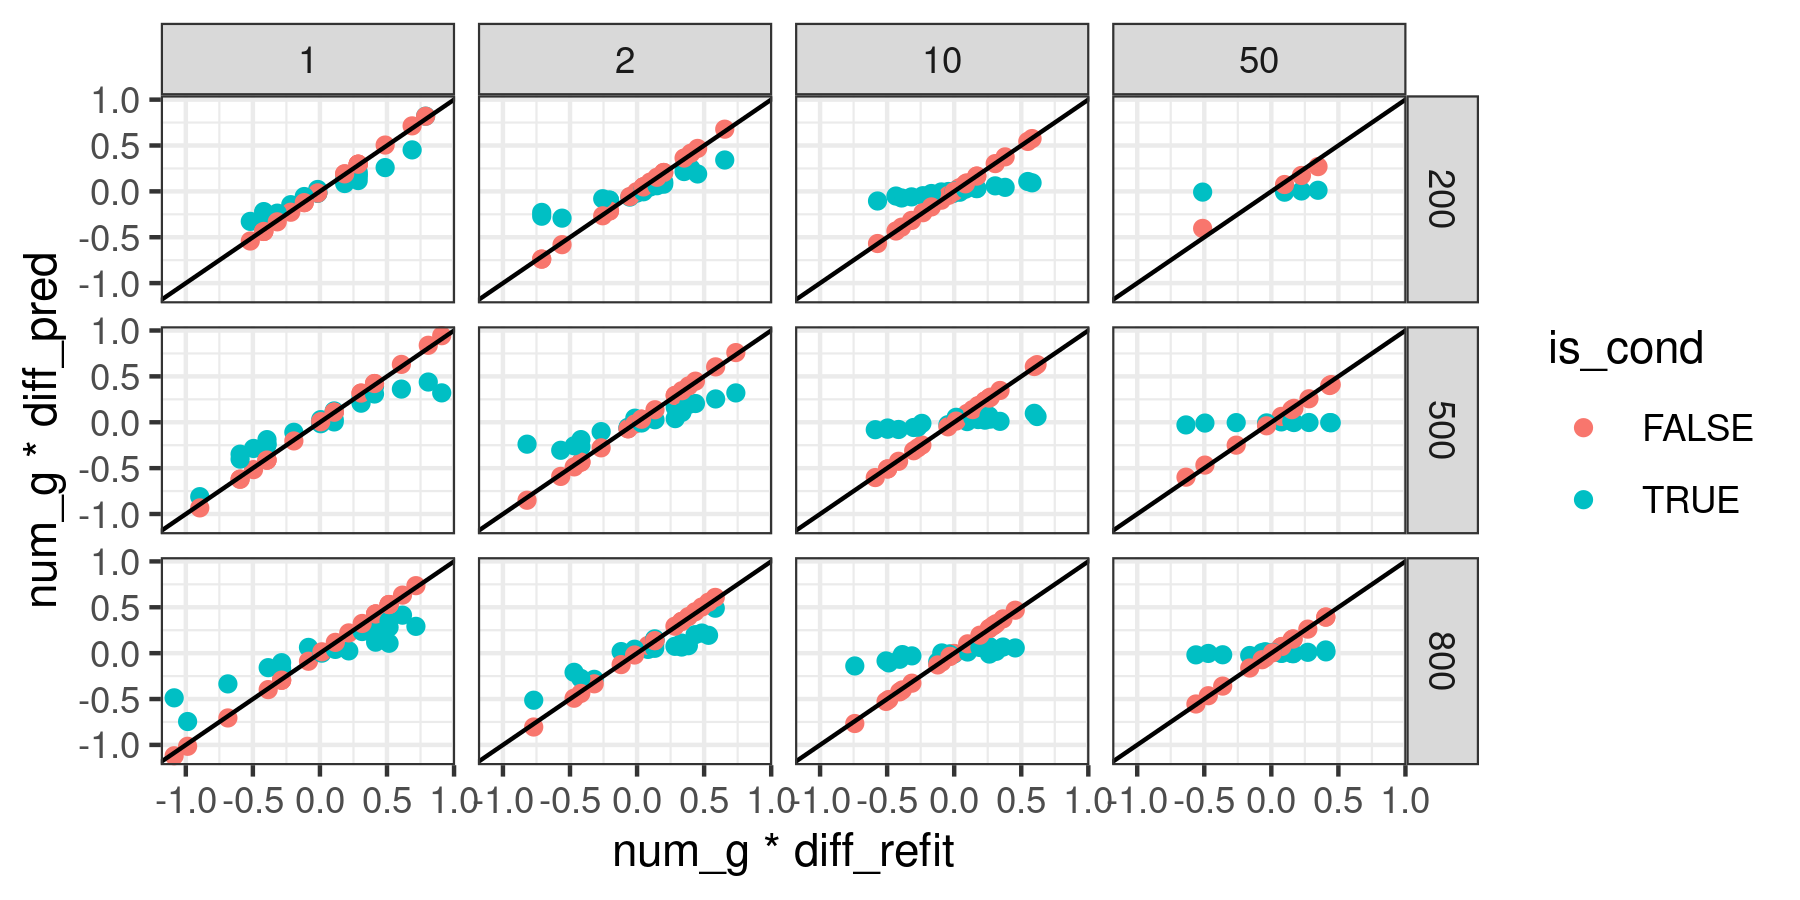
\includegraphics[width=0.980\linewidth,height=0.490\linewidth]{figure/manyplots-1} 

}



\end{knitrout}
}


\newcommand{\ManyPlotsTwo}{
%<<mult_path, cache=cache, fig.show='hold', fig.cap=fig_cap>>=
\begin{knitrout}
\definecolor{shadecolor}{rgb}{0.969, 0.969, 0.969}\color{fgcolor}

{\centering 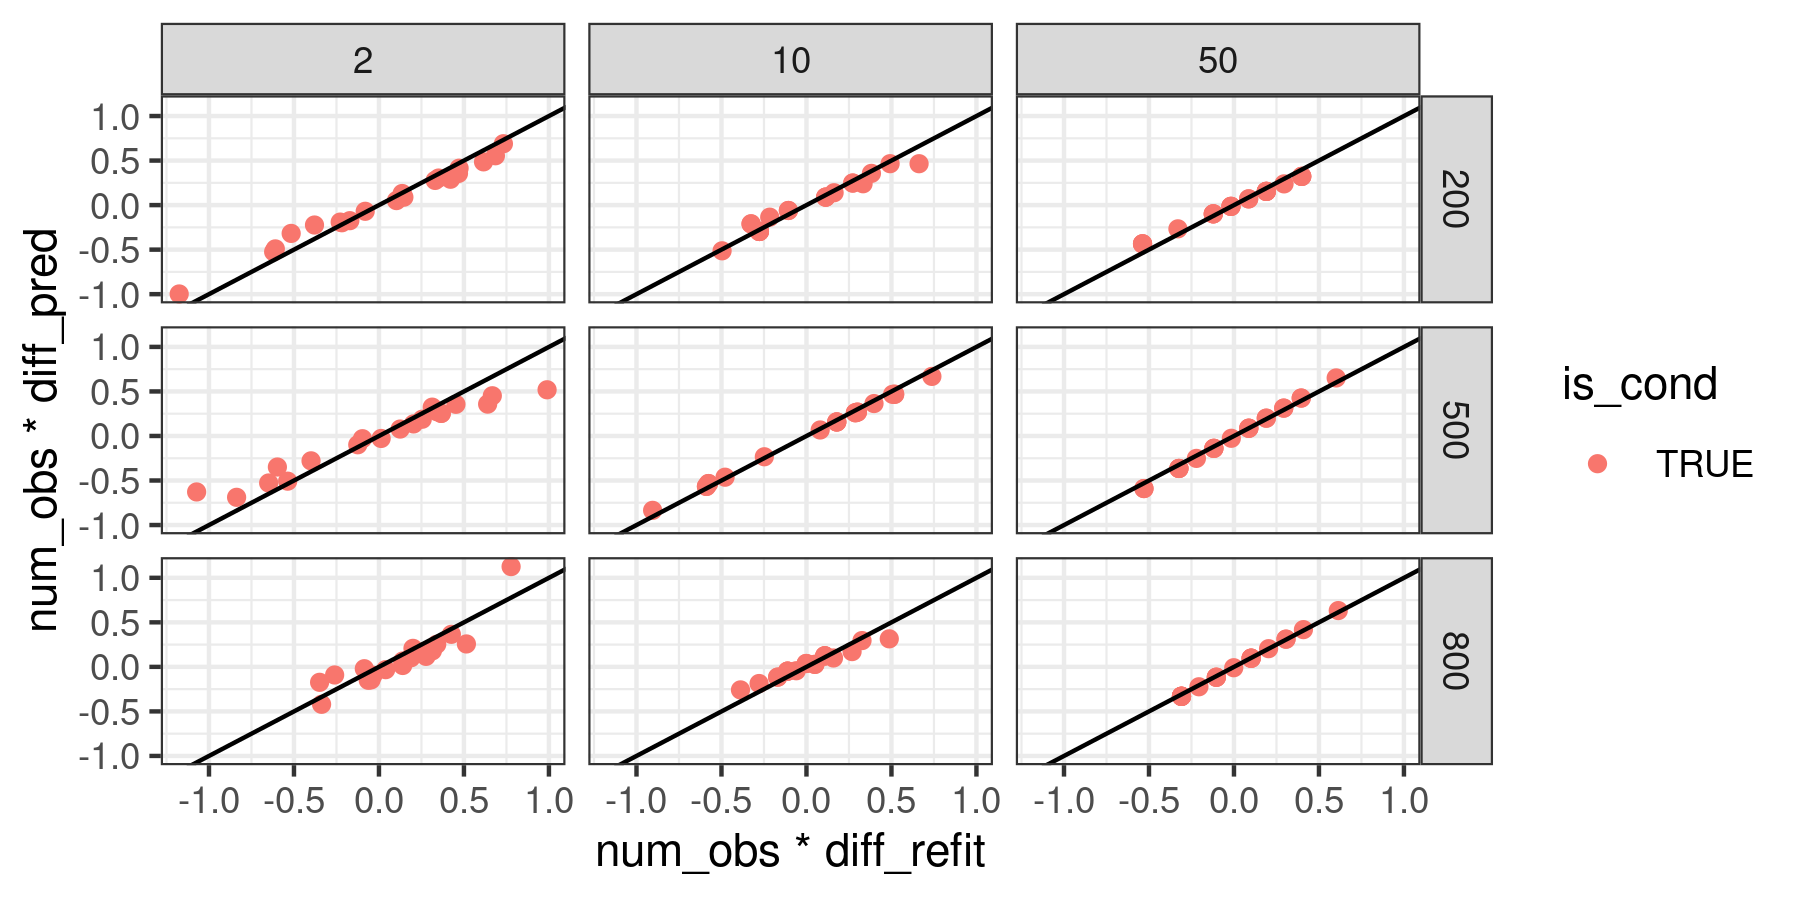
\includegraphics[width=0.980\linewidth,height=0.490\linewidth]{figure/manyplotstwo-1} 

}



\end{knitrout}
}
